\section{Supercomputers}
\label{sec:Supercomputers}

The COMPSs Framework can be installed in any Supercomputer by installing its packages as in a normal distribution. The packages are
ready to be reallocated so the administrators can choose the right location for the COMPSs installation. \newline

However, if the administrators are not willing to install COMPSs through the packaging system, we also provide a \textbf{COMPSs 
zipped file} containing a pre-build script to easily install COMPSs. Next subsections provide further information about this process.


\subsection{Prerequisites}
In order to successfully run the installation script some dependencies must be present on the target machine. Administrators must 
provide the correct installation and environment of the following software:
\begin{itemize}
 \item Autotools
 \item BOOST
 \item Java 8 JRE
\end{itemize}

The following environment variables must be defined:
\begin{itemize}
 \item $JAVA\_HOME$
 \item $BOOST\_CPPFLAGS$
\end{itemize}

The tracing system can be enhanced with:
\begin{itemize}
 \item PAPI, which provides support for harware counters
 \item MPI, which speeds up the tracing merge (and enables it for huge traces)
\end{itemize}


\subsection{Installation}
To perform the COMPSs Framework installation please execute the following commands:
\begin{lstlisting}[language=bash]
 # Check out the last COMPSs release
 $ wget http://compss.bsc.es/repo/sc/stable/COMPSs_<version>.tar.gz

 # Unpackage COMPSs
 $ tar -xvzf COMPSs_<version>.tar.gz
 
 # Install COMPSs at your preferred target location
 $ cd COMPSs
 $ ./install <targetDir>
 
 # Clean downloaded files
 $ rm -r COMPSs
 $ rm COMPSs_<version>.tar.gz
\end{lstlisting}

The installation script will create a COMPSs folder inside the given $<targetDir>$ so the final COMPSs installation will be placed 
under the $<targetDir>/COMPSs$ folder. Please note that if the folder already exists it will be \textbf{automatically erased}.

~ \newline
After completing the previous steps, administrators must ensure that the nodes have passwordless ssh access. If it is not the case,
please contact the COMPSs team at $support-compss@bsc.es$.

~ \newline
The COMPSs package also provides a \textit{compssenv} file that loads the required environment to allow users work more easily
with COMPSs. Thus, after the installation process we recomend to source the $<targetDir>/COMPSs/compssenv$ into the 
users \textit{.bashrc}.

~ \newline
Once done, remember to log out and back in again to end the installation process.

\subsection{Configuration}
For queue system executions, COMPSs has a pre-build structure (see Figure \ref{fig:queue_scripts_structure}) to execute 
applications in SuperComputers. For this purpose, users must use the \textit{enqueue\_compss} script provided in the COMPSs installation.
This script has several parameters (see \textit{enqueue\_compss -h}) that allow users to customize their executions for any SuperComputer.

\begin{figure}[h!]
  \centering
    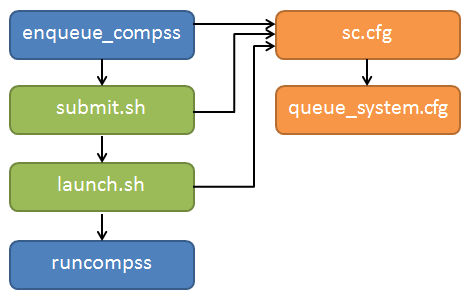
\includegraphics[width=0.6\textwidth]{./Sections/6_Supercomputers/Figures/queue_scripts_structure.png}
    \caption{Structure of COMPSs queue scripts. In Blue user scripts, in Green queue scripts and in Orange system dependant scripts}
    \label{fig:queue_scripts_structure}
\end{figure}

To make this structure works, the administrators must define a configuration file for the queue system 
(under $<targetDir>/COMPSs/scripts/queues/cfgs/QUEUE/QUEUE.cfg$) and a configuration file for the specific SuperComputer parameters
(under $<targetDir>/COMPSs/scripts/queues/cfgs/SC_NAME.cfg$). The COMPSs installation already provides queue configurations for \textit{LSF} and 
\textit{SLURM} and several examples for SuperComputer configurations. 

To create a new configuration we recommend to use one of the configurations provided by COMPSs (such as the configuration for the
\textit{MareNostrum III} SuperComputer) or to contact us at \url{support-compss@bsc.es} .

\subsection{Post installation}
To check that COMPSs Framework has been successfully installed you may run:
\begin{lstlisting}[language=bash]
 # Check the COMPSs version
 $ runcompss -v
 COMPSs version <version>
\end{lstlisting}

For queue system executions, COMPSs provides several prebuild queue scripts than can be accessible throgh the \textit{enqueue\_compss}
command. Users can check the available options by running:
\begin{lstlisting}[language=bash]
enqueue_compss -h
Usage: enqueue_compss [queue_system_options] [COMPSs_options] 
          application_name [application_arguments]

* Options:
  General:
    --help, -h                              Print this help message
  
  Queue system configuration:
    --exec_time=<minutes>                   Expected execution time of the application (in minutes)
                                            Default: 10
                                            
    --num_nodes=<int>                       Number of nodes to use
                                            Default: 2
                                            
    --num_switches=<int>                    Maximum number of different switches. 
                                            Select 0 for no restrictions.
                                            Maximum nodes per switch: 18
                                            Only available for at least 4 nodes. 
                                            Default: 0 

    --tasks_per_node=<int>                  Maximum number of simultaneous tasks running on a node
                                            Default: 16
                                            
    --node_memory=<MB>                      Maximum node memory: disabled | <int> (MB)
                                            Default: 28
                                            
    --network=<name>                        Communication network for transfers: 
                                              default | ethernet | infiniband | data.
                                            Default: ethernet

    --sc_cfg=<name>                         SuperComputer configuration file to use. 
                                            Must exist inside queues/cfgs/
                                            Default: default
                                            
    --queue=<name>                          Queue name to submit the job. Depends on the queue system.
                                            For example (MN3): bsc_cs | bsc_debug | debug | interactive
                                            Default: default
                                            
    --reservation=<name>                    Reservation to use when submitting the job. 
                                            Default: disabled
                                            
    --job_dependency=<jobID>                Postpone job execution until the job dependency has ended.
                                            Default: None

    --master_working_dir=<path>             Working directory of the application
                                            Default: .
                                            
    --worker_working_dir=<name | path>      Worker directory. Use: scratch | gpfs | <path>
                                            Default: scratch
                                            
    --worker_in_master_tasks=<int>          Maximum number of tasks that the master node 
                                            can run as worker. Cannot exceed tasks_per_node.
                                            Default: 0
                                            
    --worker_in_master_memory=<int> MB      Maximum memory in master node assigned to the worker.
                                            Cannot exceed the node_memory.
                                            Mandatory if worker_in_master_tasks is specified.
                                            Default: disabled
                                            
    --jvm_worker_in_master_opts="<string>"  Extra options for the JVM of the COMPSs Worker 
                                            in the Master Node. Each option separed by "," and without 
                                            blank spaces (Notice the quotes)
                                            Default: 
                                            
    --task_execution=<compss|storage>       Task execution under COMPSs or Storage.
                                            Default: compss
                                            
    --storage_conf=<path>                   Path to the storage configuration file
    
    --storage_name=<dataclay|hecuba>        Name of the storage platform dataClay or Hecuba.
    

  Runcompss delegated parameters:

  Tools enablers:
    --graph=<bool>, --graph, -g             Generation of the complete graph (true/false)
                                            When no value is provided it is set to true
                                            Default: false
                                            
    --tracing=<level>, --tracing, -t        Set generation of traces and/or tracing level
                                            ( [ true | basic ] | advanced | false)
                                            True and basic levels will produce the same traces.
                                            When no value is provided it is set to true
                                            Default: false
                                            
    --monitoring=<int>, --monitoring, -m    Period between monitoring samples (milliseconds)
                                            When no value is provided it is set to 2000
                                            Default: 0
                                            
    --external_debugger=<int>,
    --external_debugger                     Enables external debugger connection on the 
                                            specified port (or 9999 if empty)
                                            Default: false

  Runtime configuration options:
    --task_execution=<compss|storage>       Task execution under COMPSs or Storage.
                                            Default: compss
                                            
    --storage_conf=<path>                   Path to the storage configuration file
                                            Default: None
                                            
    --project=<path>                        Path to the project XML file
                                            Default: /opt/COMPSs/Runtime/configuration/
                                            xml/projects/default_project.xml
                                            
    --resources=<path>                      Path to the resources XML file
                                            Default: /opt/COMPSs/Runtime/configuration/
                                            xml/resources/default_resources.xml  
                                            
    --lang=<name>                           Language of the application (java/c/python)
                                            Default: java
                                            
    --log_level=<level>, --debug, -d        Set the debug level: off | info | debug
                                            Default: off

  Advanced options:
    --comm=<path>                           Class that implements the adaptor for communications
                                            Supported adaptors: 
                                             integratedtoolkit.nio.master.NIOAdaptor
                                             | integratedtoolkit.gat.master.GATAdaptor
                                            Default: integratedtoolkit.nio.master.NIOAdaptor
                                            
    --scheduler=<path>                      Class that implements the Scheduler for COMPSs
                                            Supported schedulers: 
                                             integratedtoolkit.components.impl.TaskScheduler 
                                             | integratedtoolkit.scheduler.readyscheduler.ReadyScheduler
                                            Default: integratedtoolkit.scheduler.readyscheduler.ReadyScheduler
                                            
    --library_path=<path>                   Non-standard directories to search for libraries 
                                            (e.g. Java JVM library, Python library, 
                                            C binding library)
                                            Default: Working Directory
                                            
    --classpath=<path>                      Path for the application classes / modules
                                            Default: Working Directory
                                            
    --base_log_dir=<path>                   Base directory to store COMPSs log files 
                                            (a .COMPSs/ folder will be created inside this location)
                                            Default: User home
                                            
    --specific_log_dir=<path>               Use a specific directory to store COMPSs log files 
                                            (the folder MUST exist and no sandbox is created)
                                            Warning: Overwrites --base_log_dir option
                                            Default: Disabled
                                            
    --uuid=<int>                            Preset an application UUID
                                            Default: Automatic random generation
                                            
    --master_port=<int>                     Port to run the COMPSs master communications.
                                            Only for NIO adaptor
                                            Default: 43000
                                            
    --jvm_master_opts="<string>"            Extra options for the COMPSs Master JVM. 
                                            Each option separed by "," and without 
                                            blank spaces (Notice the quotes)
                                            Default: 
                                            
    --jvm_workers_opts="<string>"           Extra options for the COMPSs Workers JVMs.
                                            Each option separed by "," and without 
                                            blank spaces (Notice the quotes)
                                            Default: -Xms1024m,-Xmx1024m,-Xmn400m
                                            
    --task_count=<int>                      Only for C/Python Bindings. Maximum number 
                                            of different functions/methods, invoked from 
                                            the application, that have been selected as tasks
                                            Default: 50
                                            
    --pythonpath=<path>                     Additional folders or paths to add to the PYTHONPATH
                                            Default: /home/cramonco/svn/compss/framework/trunk/compss
                                            
    --PyObject_serialize=<bool>             Only for Python Binding. Enable the object 
                                            serialization to string when possible 
                                            (true/false).
                                            Default: false


* Application name:
    For Java applications:   Fully qualified name of the application
    For C applications:      Path to the master binary
    For Python applications: Path to the .py file containing the main program

* Application arguments:
    Command line arguments to pass to the application. Can be empty.                                          
\end{lstlisting}

If none of the pre-build queue configurations adapts to your infrastructure (lsf, pbs, slurm, etc.) please contact 
the COMPSs team at $support-compss@bsc.es$ to find out a solution.

~ \newline
If you are willing to test the COMPSs Framework installation you can run any of the applications available at our application 
repository \url{https://compss.bsc.es/projects/bar}. We suggest to run the java simple application following the steps listed
inside its \textit{README} file. 

~ \newline
For further information about either the installation or the usage please check the \textit{README} file inside the COMPSs package. 

